\documentclass[a4paper,11pt]{article}
\usepackage[latin1]{inputenc}
\usepackage[T1]{fontenc}
\usepackage[italian,UKenglish]{babel}
%\usepackage[english]{babel}
\usepackage{graphicx}


\begin{document}

\begin{titlepage}

\begin{center}
\huge{\textbf{vme64x-core review 1}}\\
\end{center}
\vspace{17cm}
\begin{flushleft}
Author: Davide Pedretti
\end{flushleft}
\vspace{1cm}
\begin{flushright}
Date: 12/11/2012
\end{flushright}
\end{titlepage}
\newpage 

\begin{center}
\LARGE{\textbf{Carlos}}
\end{center}
\begin{itemize}
\item \textit{(m) Reference the AM table (line 75) to a document...}\\
Done. Hex code added as comments.
\item \textit{(?)If all the operations are controlled by DS lines (and others), 
is it necessary to place double or triple buffering in the address and data 
lines?} \\
Good observation: It is possible place triple buffering only in the control
lines: VME\_GA\_i, VME\_AS\_n\_i, VME\_WRITE\_n\_i, VME\_DS\_n\_i, VME\_RST\_n\_i, VME\_IACK\_n\_i, VME\_IACKIN\_n\_i.\\
Indeed when the vme64x core latches the address and data lines, they should be stable according with the VME specification.
\item \textit{(o) Remove use IEEE.numeric\_std.unsigned; redundant}\\
Done.
\item \textit{(?) VME\_RST\_n\_i what for?}\\
The Power Monitor Module (A20 MEN in our case) should drive this line.
See page 200 VMEbus specification ANSI/IEEE STD1024-1987.
\item \textit{(?) Debug leds should be removed?}\\
Yes. The leds were used during the debug. 
\item \textit{(o) In the same process the when others => clause is missing. 
             Probably it would be better set a deferred output before the case, 
             so it will always set an output}\\
Assigned a default configuration before the case.\\
Added when others =>.
\item \textit{(o) Coming back to the process in line 243, the previous comment 
is applicable.  Recommend to preassign before the case to avoid unwanted latches
}.\\
Assigned a default configuration before the case.\\
Added when others =>.

\item \textit{(\_) In the process in line 317, it would be better have records that
       which are assigned with predefined record constants. It will reduce the
       length and possible errors while assigning values to the outputs}.\\
Done.
\end{itemize}
\newpage
\begin{center}
\LARGE{\textbf{Javier}}
\end{center}
\begin{itemize}
\item VME\_bus.vhd\\
\textit{
There is a comment at line 527 saying:
-- If the S\_FPGA will be provided to a core who drives these lines
-- without
-- erase the A\_FPGA the above mentioned lines should be changed to 'Z'
-- !!!
This should probably change to become a generic so that people can
decide on the behaviour they want. It will then be more visible, not
hidden in the middle of the code. The sentence itself it quite
cryptic. This core should not assume it is used in a board with a
S\_FPGA and a A\_FPGA.}

The comment is related to the SVEC board, so it has been removed from the middle
of the code and 
it has been moved on the general description at the beginning of the file.\\

Each VME board plugged in a slot acts as a VME salve module and it has only one 
CR/CSR space (conforming with the specification) so only one FPGA at time 
must drive the output lines on the VME bus; only one FPGA at time can carry the 
vme64x core.\\
In other words, only one FPGA at a time shall answer to the software.\\

\item \textit{VME\_IRQ\_Controller.vhd}
\begin{itemize}
\item \textit{Text diagram in the initial comments not clear regarding state
IACKOUT2}\\
Added comment: \\
If the slave module does not have an interrupt pending (IDLE state) and it 
receives a falling edge on the IACKIN, it shall pass the falling edge through the
daisy chain. To obtain this the IACKOUT2 state has been added.
\item \textit{To avoid the time constraint" -> "To respect the timing
constraint}\\
Corrected
\item \textit{Signal naming is not consistent. If the "s\_" prefix is used, it 
should be used for all internal signals.}\\

Done. The prefix s\_ is used for all internal signals.
\item \textit{Line 104: "reset" is clearly used as an active-low signal in this
entity, and it is an input port, so its name should be "reset\_n\_i".}\\
Done. reset => reset\_n\_i.
\item \textit{Instantiation of many FlipFlopD components: a single clocked 
process would be more compact and easier to understand.}\\

FlipFlopD components replaced by a single clocked process.
\item \textit{Line 247: why should the interrupt controller not be allowed to 
go to the IRQ state when VME\_IACKIN\_n\_i='0'?}\\
If VME\_IACKIN\_n\_i='0' and the finite state machine is still in IDLE it means 
that we do not have interrupt request pending and this is not the responding 
Interrupter and so it passes the falling edge on the IACKOUT on the daisy chain.
As soon as the IACKIN has been released the finite state machine come back to the
IDLE state and it is allowed to go in the IRQ state and request service to the 
software.

\item \textit{Line 256: once we have allowed going to the IRQ state even if
VME\_IACKIN\_n\_i is low, we should detect a falling edge of
VME\_IACKIN\_n\_i while in the IRQ state to proceed. A simple detection
of '0' won't work anymore}\\

We go the IRQ state only if VME\_IACKIN\_n\_i is '1'. Once we have allowed
going to the IRQ state we wait until the VME\_IACKIN\_n\_i signal is '0'.
When it is '0' it means that the Interrupt Acknowledge Cycle is in progress and 
the finite state machine go in the WAIT\_AS state. At this point we do not need 
anymore the detection of '0' on the VME\_IACKIN\_n\_i signal.
I hope I have answered the question.

\item \textit{Line 321: In the IDLE state this block should drive whatever it 
gets from IACKIN into IACKOUT. Otherwise it is blocking interrupt
acknowledgement for any cards to the right of the module where it is
instantiated}\\

Indeed when in IDLE, if the VME\_IACKIN\_n\_i is '0' the finite state machine 
goes in the IACKOUT2 state where it drives the VME\_IACKOUT\_n\_o.\\

\textit{Driving IACKOUT with AS as is done in other
states looks weird. IACKOUT should be driven by IACKIN when the IACK
chain is not intercepted by this block.}\\

The VMEbus specification tells us that if this is not the responding Interrupter
it shall pass the falling edge of IACKIN* to the next interrupter module in the daisy chain by driving IACKOUT* low.\\

The timing rule 38A (page 183 VMEbus specification) tells us that the Interrupter can take as time it wants before asserting the IACKOUT (because before passing the falling edge the Interrupter has to check if it is the responding Interrupter). Since the timing rule 34 (in the above mentioned page) tells us that the AS* signal is asserted before the IACKIN*, the Interrupter implemented drives the 
IACKOUT* with the AS* instead of the IACKIN*. In so doing the Interrupter developed matches the timing rule 35 also at low frequencies.\\ See page 6.

\item \textit{Line 445: these are active-low signals so their value after reset
should be '1', not '0'}.\\

After reset the VME\_IRQ\_n\_o lines are already set to '1'.

\item \textit{I don't understand the whole DS\_LATCH thing. We detect in state
WAIT\_DS that there was some change in the DS lines. This makes us go
to state LATCH\_DS, where the DS lines are latched. Then we check if
VME\_DS\_latched(0) is '0' in the ACK\_INT state. Wouldn't it be simpler
to just wait for DS(0) to become '0'?}\\

In our system the Interrupt Handler supports the data transfer type D08(O) and during the Interrupt Acknowledge Cycle the DS1 line is never asserted (always '1') so it is possible delete the LATCH\_DS state and 
delete the further control VME\_DS\_latched(0) = '0' in the ACK\_INT state.

More in general, the type of Interrupter can be also D32. In this case (as shown in the table 31 page 157 VMEbus specification) the Interrupter shall monitor also the DS1* and the LWORD* lines. When I started to implement the Interrupter I did not know in which way the Interrupt Handler was working so I added the LWORD* (never used at the moment) and DS1* lines.

If a D32 interrupter will be used, the finite state machine should be provided with one or more LATCH\_DS states  to match the timing rule 13, as done in the VME\_bus component.

The vhdl file has been changed in order to be less confusing. The VME\_DS\_latched(0) = '0' control has been deleted since it was redundant in any case.

\item \textit{Line 467: s\_enable opens the sampling gate for INT\_Req only when
either we have not latched a request (with INT\_Req\_sample) or when
DTACK is being driven low. In this last case, we are in the DTACK
state (until AS goes up) and any INT\_Req pulse will go through the
sampling but in a transient way, i.e. it will not "stick" and we will
lose it. This behavior should be documented so that users of the core
know.}\\

This behavior is undesired. The IRQ\_Controller has been corrected
but in any case interrupt requests coming from the WB application before the Interrupter detects the end of the Interrupt Acknowledge Cycle (AS* rising edge), are lost. 
The Interrupter implemented has no queue.

\item \textit{VME\_AS\_n\_i and VME\_DS\_n\_i are passed to two different synchronizer
blocks in parallel. The actual implementation of this will depend on
how clever the synthesis tool is. If it is not clever, it will not
notice it can tap the three-FF synchronizer to get the double-FF
output, and we will have two parallel synchronizers: not good,
especially considering that one of them will not use the I/O FFs. If
these double-clocked signals are really needed, the triple-clocking
block could deliver an extra ouput port for them.}\\

Done.

\end{itemize}
\end{itemize}
\newpage
\begin{center}
\LARGE{\textbf{Pablo}}
\end{center}
\begin{itemize}
\item VME\_IRQ\_Controller.vhd\\
\textit{(m!) As it is already pointed out by Javier the IACKIN-IACKOUT should be looked in more detail. I doubt the interrupt 
handler can deal correctly with rule 4.41 (30ns min skew between AS release and IACKOUT release). Notice that this rule applies on the VME connector edge so even with an internal latency of 2 cycles at 10ns you still have all the propagations delays to take care of}\\

Rule 4.41: A partecipating interrupter shall drive IACKOUT* high within this maximum time after the rising edge on AS*.\\
Please note that this rule refers to the interrupter not to the interrupt handler. The figure 55 (page 183 VMEbus specification)
and the related table tell us that the Interrupt Handler does not care the time 35 (so why should we care about that?).\\

However, as you said, if this rule applies on the VME connector edge we are not matching it.
If we drive the IACKOUT* with the IACKIN* as Javier suggested, we do not match this timing rule because of the timing rule 39.
Thus, the only way to always match this rule, regardless of the clock frequency used, is drive the IACKOUT* signal with the AS*
signal not sampled. The metastability will not be a problem in this case because when this signal is outputted it is 
already stable.
\item VME\_bus.vhd\\
\textit{(m) It was pointed out in the presentation that the DS toggle could eventually not be properlly detected. In the datasheet it is stated that the skew between this lines can be up to a maximum of 20ns. A single wait state may be not enough if the vme core is clocked at 100MHz. On the other hand it is not necessary if the core is clocked at f<50Mhz. Probably it could be a good idea to use some generic (as carlos sugested) to insert/remove wait states depending on the clocking frequency}\\

Done.\\
Now, in the main finite state machine there are up to 4 LATCH\_DS states selectable with a generic paramiter: g\_clock.
It means that now the timing rule 2.39 page 113 (VMEbus specification ANSI/IEEE STD1014-1987) can be matched up to 200 MHz by 
setting the generic g\_clock with the clock period in ns.\\
Adding other LATCH\_DS states the rule 2.39 can be met with frequencies upper to 200 MHz.\\
\begin{itemize}
\item 50 MHz or less: only 1 LATCH\_DS state
\item from 50 MHz to 100 MHz: 2 LATCH\_DS states.
\item from 100 MHz to 150 MHz: 3 LATCH\_DS states.
\item from 150 MHz to 200 MHz: 4 LATCH\_DS states.
\end{itemize}
Please note that in order to meet the timing rule 2.31 (\textit{When using the DTB for two consecutive cycles, the master shall 
not drive AS* low until it has been high for this minimum time (30 ns for the slave))} we suggest to use the vme64x core with 
frequencies upper than 40 MHz. To match this rule with lower frequencies it is necessary to use different clock domains, and so 
a FIFO, inside the vme64x core and sampling the input signals with frequencies upper than 40 MHz.

\end{itemize}
\newpage

\begin{center}
\LARGE{\textbf{Tom}}
\end{center}
\begin{itemize}
\item VME\_bus.vhd\\
\textit{(m) don't comment out code that is not used. Just remove it.}\\
Done
\item VME\_IRQ\_Controller.vhd\\
\textit {(!) line 235: is reset signal active low or high?}\\
As Javier suggested the reset has been renamed reset\_n\_i.
\item VME\_CR\_CSR\_Space.vhd\\
\textit{(m) GADER\_1 loop: please put a single-line comment describing what the generate loop does.}\\
Done.\\
It generates a vector of 8 array (unsigned 32 bits).\\
We need these registers in the decoder.
\item VME\_Access\_Decode.vhd\\

\textit {(o) provide a generic allowing for reduction of device functions. In most cases, we need only 1 A24/A32/D32 BAR.
  Decoding and storing BAR configurations takes large percentage of the FPGA resources consumed by the VME core.}\\

I think you can discuss about this point with Julian and David. At the moment I prefer provide the CR/CSR space with all the
functions according with the specification. The aim is to provide you a generic vme64x slave module in agreement with the 
specification. You can change the CR/CSR space in order to obtain a custom vme64x slave module at a later time.\\

\textit {(!) process driving cardsel and base\_addr: sequential nonblocking assignments are potentially
  dangerous - you are relying on assumption that if any of bits in s\_func\_sel is 1, cardsel (previously set
  to 0) will be overwritten by the loop. It's safer to use variables and blocking assignments in such cases.}\\

According to the section 8.7 of the \textit{VHDL for logic synthesis} Third edition, this process is synthesized as shown in the 
following figure:\\
\newpage
\begin{figure}[ht]
\begin{center}
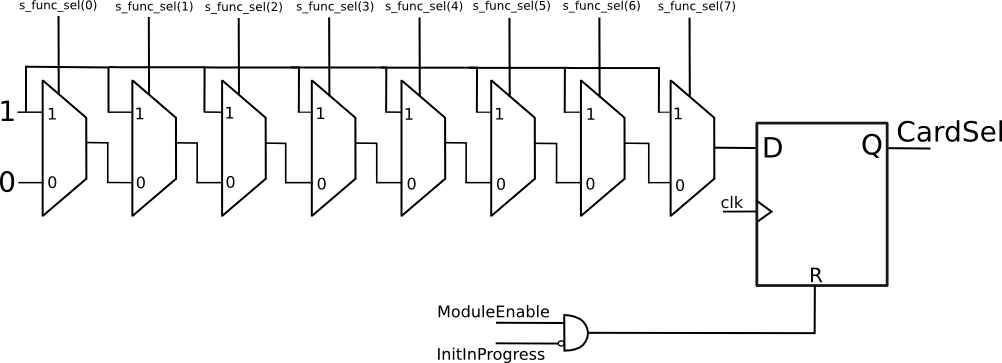
\includegraphics[scale=0.70]{for_loop}
\end{center}
\end{figure} 

I checked the RTL Schematic after synthesis and, the Base\_Addr and CardSel are synthesized as shown in the above image. \\
I deleted the exit statement that is useless in this case.\\
Thus, the process has not been changed.
\item VME64xCore\_Top.vhd\\
\textit {(\_) Process at lines 530+: I would place it in VME\_bus. This way the top level module will only
  act as an interconnect putting together all VME core components.}\\
Done.
The process can be found in the VME\_Wb\_master.vhd component.

\end{itemize}
\newpage
\begin{center}
\LARGE{\textbf{Thedi}}
\end{center}

\begin{itemize}
\item You can find the c\_SIZE constant in the genram\_pkg.\\
\item I developed the code with the Xilinx ISE tool so if you open the code with another editor it may be unaligned.
\item \textit{line 316: this is actually a Moore FSM (outputs depend only on current state)}\\
In the sensitivity list of the project there is also the AS* signal so I wrote: Mealy FSM
\item \textit{I suggest you put the constant values in hex. They are a lot more
readable than binary}.\\
The constant are in binary because each bit corresponds to one AM. These are mask bits.
It is easy to change them in binary.\\
The best thing can be to create a function which takes the AMs as arguments and sets them automatically.
\item \textit{I personally find it a bad idea to define multiple components in the same file.
When I get an entity name in an instantiation, my first instinct is to start
looking for a file with the same name as the entity.}\\

Yes it is not a good idea but also create a file for each small entity it is not nice. These entity are
double flopping, triple flopping, rising and falling edge detection so are all grouped inside one file.\\
\item I corrected some English errors. For sure there are other errors. Apologize my English! :) 
\end{itemize}
\newpage

\begin{center}
\LARGE{\textbf{Matthieu}}
\end{center}
\begin{itemize}
\item \textit{Change MBLT endian register name to SWAP configuration register 
(or something similar).}\\
Done.\\
MBLT Endian register renamed Endian since it can be used during all the access 
modes except during the CR/CSR accesses.
\item \textit{Add a reset output port on core's top level.}\\
In the VME64xCore\_Top's output port there is already a reset\_o signal which is active high and it comes from the software reset bit in the CRS space.
\item I deleted some of the not used signals.
\item \textit{Update the Manifest file.}\\
Done
\item now, you should not see same of the warnings you indicated to me in your 
review.
\end{itemize}
\newpage
In the VME64xCore\_Top.vhd file it is possible to find the following generic paramiters:\\
\begin{itemize}
\item g\_clock
\item g\_wb\_data\_width.
\item g\_wb\_addr\_width.
\item g\_cram\_size.
\item g\_BoardID.
\item g\_ManufacturerID.
\item g\_RevisionID.
\item g\_ProgramID.
\end{itemize}

In the VME\_IRQ\_Controller.vhd component, the ACK\_INT state has been renamed CHECK; less confusing\\

During this first review I focused more on the timing problems, not synthesizable processes and so on.
I started from the (!) serious and (m) medium advices and I tried 
to answer all the questions. \\
I deleted more or less all the never used signals and processes related to the 2emodes and the buffer not implemented. In so doing the project is less 
confusing and clearer.\\
I tested again the vme64x core after making changes and it is still working fine.\\
I cannot see further timing rules violated.\\


\end{document}

